% !TEX root = ../thesis_main.tex
\chapter{Prior Ultrafast Spectroscopy Studies of SWCNTs}

\section{Overview}

{\color{red} UNFINISHED} Want to make lasers. Need population inversion. Not possible to achieve if nonlinear processes such as exciton-exciton annihilation or Auger scattering occur. Conflicting reports regarding whether exciton-exciton annihilation in CNTs actually occurs.

\section{Inter-band and Inter-subband Recombination Dynamics}

{\color{red} ADD INTRO PARAGRAPH FOR THIS SECTION}

\subsection{Ostojic et al. (2004)}
Ostojic et al.\ (2004) presented an early work regarding the carrier recombination dynamics of carbon nanotubes \cite{ostojic2004interband}. They conducted wavelength-dependent, degenerate pump-probe measurements using an optical parametric amplifier with a time resolution of $\sim$150 fs (See Section \ref{section:opa} for details regarding the function of optical parametric amplifiers) whereby the pump and probe have the same photon energy. The sample they studied consisted of a dispersion of HiPCo SWCNTs (See Sections \ref{section:cnt_synthesis} and \ref{section:dispersion_swcnt} for details).

\begin{figure}[ht]
	\centering
	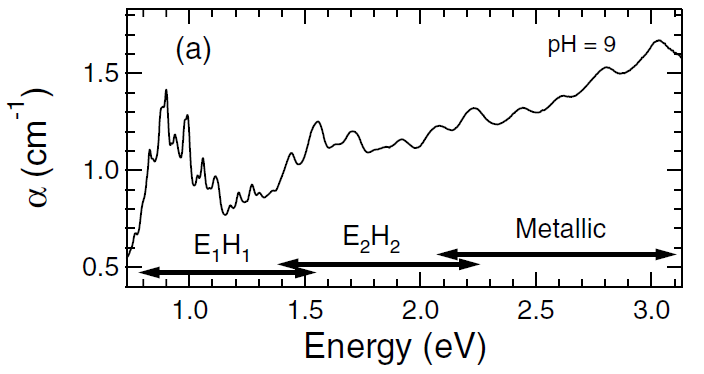
\includegraphics[scale=0.7]{images/chapter_prior_works/abs_gordana}

	\caption{Optical absorption spectrum of dispersed HiPCo SWCNTs studied by Ostojic et al.\ (2004). The spectrum contains optical resonances associated with semiconducting nanotubes which include $E_{11}$ in the region denoted as $E_{1} H_{1}$ as well as  $E_{22}$ in the region labeled as $E_{2} H_{2}$. The remaining resonances in the Metallic region come from the $E_{11}$ resonances of metallic nanotubes. Reproduced and modified from Ref.\ \cite{ostojic2004interband}.}
	\label{fig:abs_gordana}
\end{figure}


Figure \ref{fig:abs_gordana} shows the optical absorption spectrum of their sample which indicates the presence of many different chiralities, including both metallic and semiconducting nanotubes. The spectral region spanning $E_{1} H_{1}$ contains optical resonances associated with the $E_{11}$ transition occurring in semiconducting nanotubes. The region defined as $E_{2} H_{2}$ contains $E_{22}$ transitions of semiconducting nanotubes. Finally, the region defined as Metallic exhibits the remaining $E_{11}$ resonances emerging from metallic nanotubes.

\begin{figure}[ht]
	\centering
	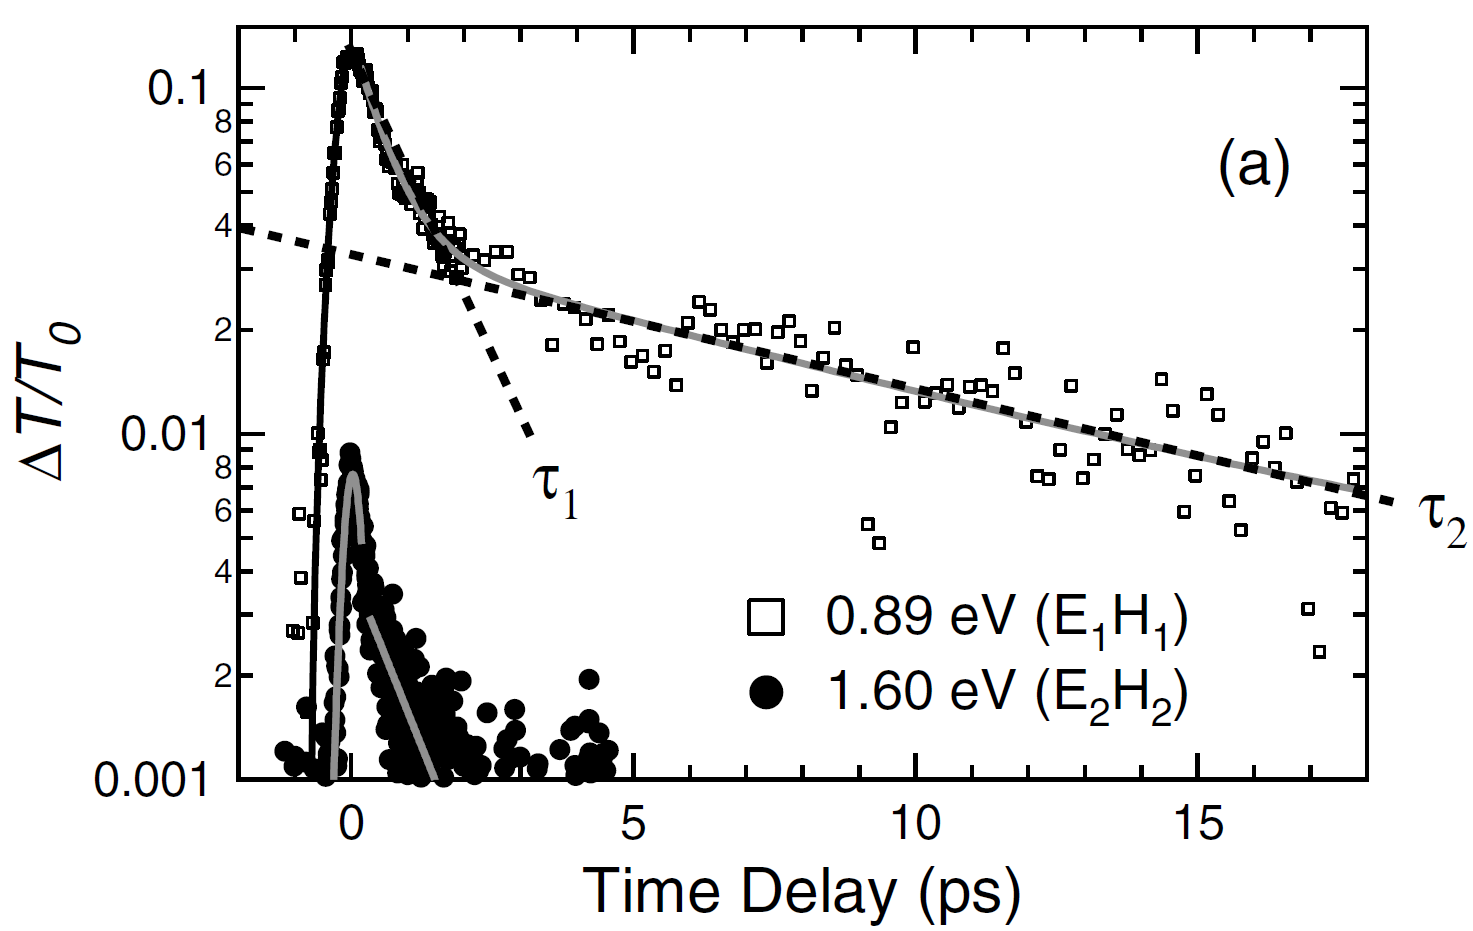
\includegraphics[scale=0.3]{images/chapter_prior_works/dtt_gordana}
	\caption{Differential transmission data at photon energies 0.89 eV (white squares) and at 1.60 eV (black circles) obtained from degenerate pump-probe measurements. At 1.60 eV, only a single exponential decay process associated with intra-band relaxation is observed. At 0.89 eV, a bi-exponential decay occurs. The fast and slow components of the bi-exponential decay are associated with intra-band and inter-band dynamics respectively. Reproduced and modified from Ref.\ \cite{ostojic2004interband}}
	\label{fig: abs_gordana}
\end{figure}

The observed carrier dynamics showed a clear wavelength dependence as shown in Figure \ref{fig:dtt_ph_gordana}. For pumping and probing within the $E_2 H_2$ region, carrier was best described by a single exponential decay process which was interpreted as intra-band relaxation to lower-energy states. In contrast, a bi-exponential decay process was observed when pumping and probing in the $E_1 H_1$ region. The initial, fast decay was interpreted as intra-band relaxation. However, the following slow exponential decay process was interpreted as inter-band relaxation. At the time of publication, this slow exponential decay process had not been observed before.

Ostojic et al.\  also note that for any chosen wavelength in their degenerate pump-probe study, some nanotubes are resonantly excited whereas others are photo-excited in a non-resonant fashion. This can affect the observed carrier decay dynamics. Figure \ref{fig:wl_dep_gordana} demonstrates this behavior. When photo-exciting the sample at an optical resonance, the ratio between the slow and fast decay times reaches a local maximum. In contrast, when pumping at spectral regions that do not exhibit a well-defined resonance, this ratio diminishes.

\begin{figure}[ht]
	\centering
	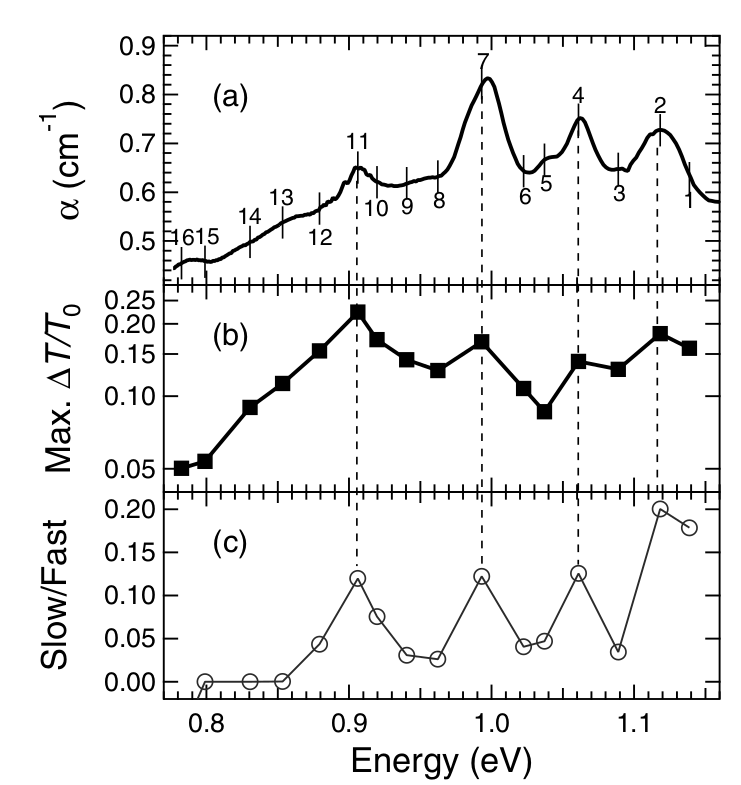
\includegraphics[scale=0.3]{images/chapter_prior_works/wavelength_dependence_gordana}
	\caption{(a) Optical absorption spectrum of the HiPCo SWCNT dispersion. The labeled positions indicate photon energies at which pump-probe measurements were taken. (b) Maximum differential transmission recorde at each measured photon energy. Differential transmission appears to reach a local maximum when the photon energy matches an optical resonance. (c) Ratio between the slow and fast decay times at each measured photon energy. The slow decay time reaches a local maximum when pumping at an optical resonance. Reproduced and modified from Ref.\ \cite{ostojic2004interband}}
	\label{fig:wl_dep_gordana}
\end{figure}

Hence, resonant excitation enhances the appearance of inter-band recombination dynamics. However, non-resonant excitations are more associated with the fast intra-band dynamics. This suggests that the reported decay times only yield statistical averages of the carrier lifetime of the ensemble of all nanotubes that have optical resonances at energies less than or equal to the pump photon energy. Furthermore, they acknowledge that they did not observe a clear correlation between the power of the optical pump and the observed carrier decay times. This excludes the observation of any nonlinear, nonradiative recombination mechanisms such as Auger recombination or exciton-exciton annihilation.

\begin{figure}[ht]
	\centering
	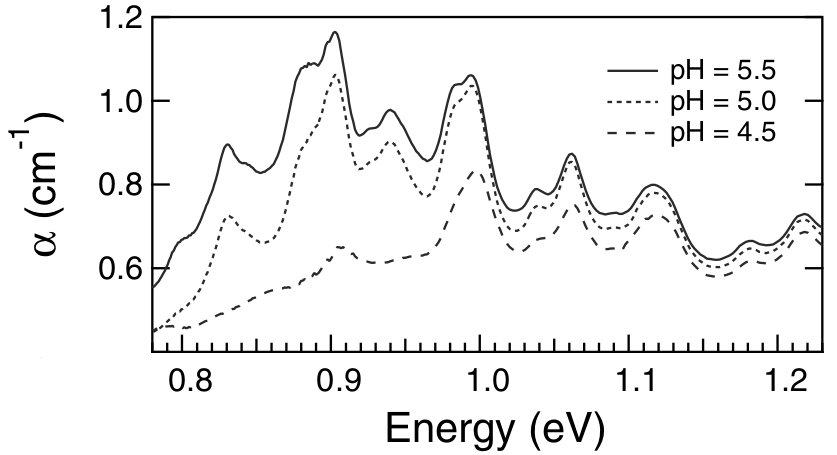
\includegraphics[scale=1.5]{images/chapter_prior_works/ph_effect_gordana_revised}
	\caption{The effect of pH on linear absorption. As the pH reduces from 5.5 to 4.5, absorption peaks at lower photon energies become supressed. This occurs as a consequence of the Burstein-Moss effect, as H$^+$ ions act as dopants that accept electrons. These dopants primarily affect larger-diameter nanotubes, as they exhibit lower binding energies for acceptors in light of their smaller effective masses. Reproduced and modified from Ref.\ \cite{ostojic2004interband}.}
	\label{fig:ph_abs_gordana}
\end{figure}

Decreasing the pH of the sample was observed to suppress optical absorption peaks, especially those occurring at lower photon energies as shown in Figure \ref{fig:ph_abs_gordana}. Correspondingly, the presence of the slow exponential decay process also diminished as shown in Figure \ref{fig:dtt_ph_gordana}. These effects were understood as a consequence of the Burstein-Moss effect. In other words, H$^+$ ions of the acidic aqueous suspension dope suspended SWCNTs by accepting negatively-charged carriers. This positions the Fermi level primarily within the valence band for nanotubes with larger diameters due to their smaller acceptor binding energies associated with their smaller effective masses.  As a result, the appearance of an inter-band absorption peak diminishes which subsequently removes the possibility of enhancing the occurrence of the inter-band relaxation by photo-exciting at well-defined optical resonances.

\begin{figure}[H]
	\centering
	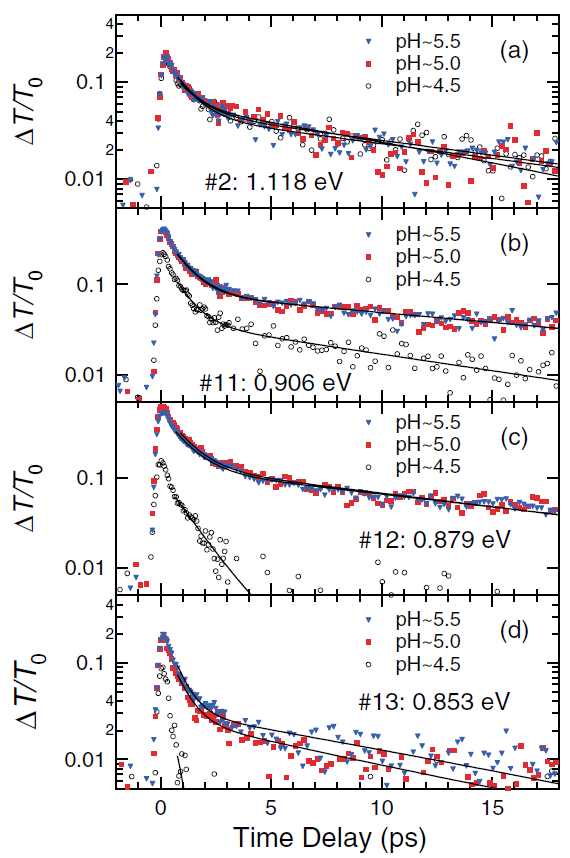
\includegraphics[scale=0.5]{images/chapter_prior_works/dtt_ph_gordana}
	\caption{The effect of pH on the carrier dynamics of nanotubes. Each plot corresponds to a degenerate pump-probe experiment conducted at a specified photon energy. As pH decreases, nanotubes become increasingly doped with positively-charge carriers. This has a larger effect on larger-diameter nanotubes due to their lower acceptor binding energies and lower the Fermi level into the valence band. At lower photon energies, the inter-band recombination process does not appear as the optical resonances associated with this process become supressed. Reproduced and modified from Ref.\ \cite{ostojic2004interband}}
	\label{fig:dtt_ph_gordana}
\end{figure}



\subsection{Manzoni et al.\ (2005)}
Manzoni et al.\ (2005) investigated the inter-subband dynamics of SWCNTs using non-degenerate pump-probe measurements with a time resolution of 40 fs. They used two OPAs to generate pump and probe pulses respectively. Furthermore, the sample they studied was a nanotube film made using HiPCo SWCNTs. Figure \ref{fig:abs_manzoni} shows the optical absorption spectrum of this sample along with the specta of the pump pulses used in this study. The sample contains a variety of optical resonances that belong to semiconducting and metallic nanotubes. The spectral regions labeled as EX1, EX2, and EX3 indicate $E_{11}$, $E_{22}$, and $E_{33}$ resonances of semiconducting nanotubes respectively. The region marked as Metallic shows the $E_{11}$ resonances for metallic nanotubes.

Depending on the pump and probe photon energies, the observed carrier relaxation dynamics either exhibit photo-induced transsmission or photo-induced absorption. For instance, Figure \ref{fig:e11_pump_manzoni} shows the experimental results obtained when pumping in the EX1 region at 0.92 eV. The differential transmission signal probed at 0.95 eV shows clear signs of photo-bleaching which indicates a finite population of photo-excited carriers. In contrast, the dynamics probed at 2 eV indicate the presence of photo-induced absorption.

\begin{figure}[H]
	\centering
	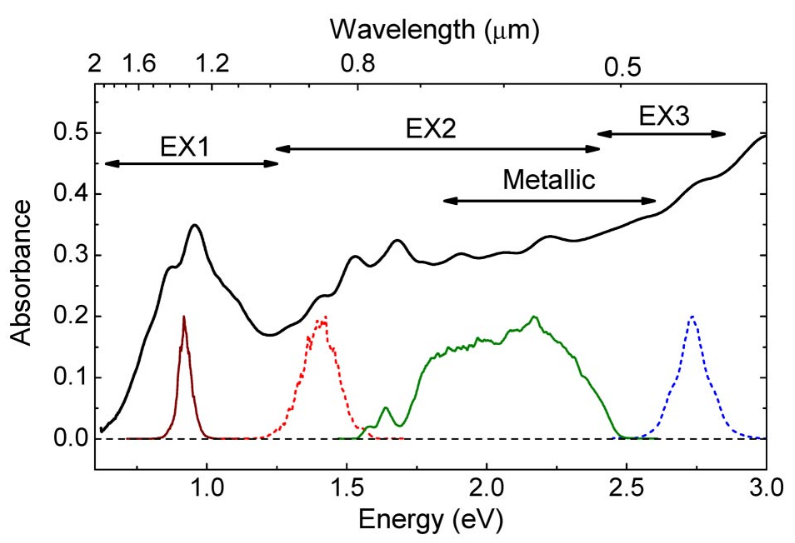
\includegraphics[scale=0.4]{images/chapter_prior_works/abs_manzoni}
	\caption{The black, solid line up top shows the absorption spectrum of HiPCo SWCNT film studied by Manzoni et al. (2005). The spectral regions indicated as EX1, EX2, and EX3 contain the $E_{11}$, $E_{22}$, and $E_{33}$ transitions of semiconducting nanotubes respectively. The region labeled as Metallic contains the $E_{11}$ resonance of metallic nanotubes. The plots shown below represent the spectra of optical pump pulses used to photo-excite the SWCNT sample in this study. Reproduced and modified from Ref.\ \cite{manzoni2005intersubband}.}
	\label{fig:abs_manzoni}
\end{figure}

Photo-bleaching does not occur due to the fact that the photon energy of the pump is below photon energies of the resonances in EX2. Hence, this photo-induced absorption was interpreted to occur due to an inter-subband transition between a state in the EX1 region and another appropriate state located in EX3 as the energy difference between two such states would be on the order of 2 eV. Additionally, this probe signal at 2 eV exhibits an oscillatory component that was attributed to a radial breathing mode (RBM) of semiconducting CNTs that occurs at a frequency of 259 $\text{cm}^{-1}$. From examining Raman spectra, this indicated that SWCNTs such as (10,3), (11,1), (9,4) and (9,4) were photo-excited in this measurement.


When exciting the SWCNTs at an energy of 2.15 eV in the EX2 region, different dynamics occurred as shown in Figure \ref{fig:e22_pump_manzoni}. Photo-bleaching occurred at the probed photon energy of 0.95 eV. In addition, both photo-induced and transmission and absorption occurred at the probed photon energy of 2.15 eV. The initial photo-bleaching indicates a finite population of $E_{22}$ excitons. Furthermore, the decay occuring afterwards indicates the relaxation from $E_{22}$ to $E_{11}$. This process occurs on a time scale of 150 fs with an associated exponential decay constant of $\sim$40 fs. The photo-induced absorption was again interpreted to occur due to a possible transition between an EX1 state and an EX3. An oscillatory signal was also observed here which was associated with an RBM frequency of 246 $\text{cm}^{-1}$ linked with nanotubes such as (10,3), (9,5), (9,4), and (7,6).


Figure \ref{fig:e33_pump_manzoni} illustrates the effect of photo-exciting at 2.75 eV (EX3) and probing at 2.1 eV (EX2). Under these conditions, a small photo-bleaching signal followed by photo-induced absorption occurred. This demonstrated the fast relaxation dynamics from EX3 states into EX1 states. Furthermore, the time constant for this process found to be $\sim$65 fs. Following the previous observations, the photo-induced absorption observed at EX2 also indicated the carrier occupation of EX1 states.

Finally, Manzoni et al.\ mentioned that they observed a weak relationship between optical pump intensity and observed recombination dynamics as shown in the inset plot of Figure \ref{fig:e22_pump_manzoni}. At higher pump intensities, the time constant for the exponential decay did not change in a significant fashion. Thus, they did not observe exciton-exciton annihilation in their studies.

\begin{figure}[H]
	\centering
	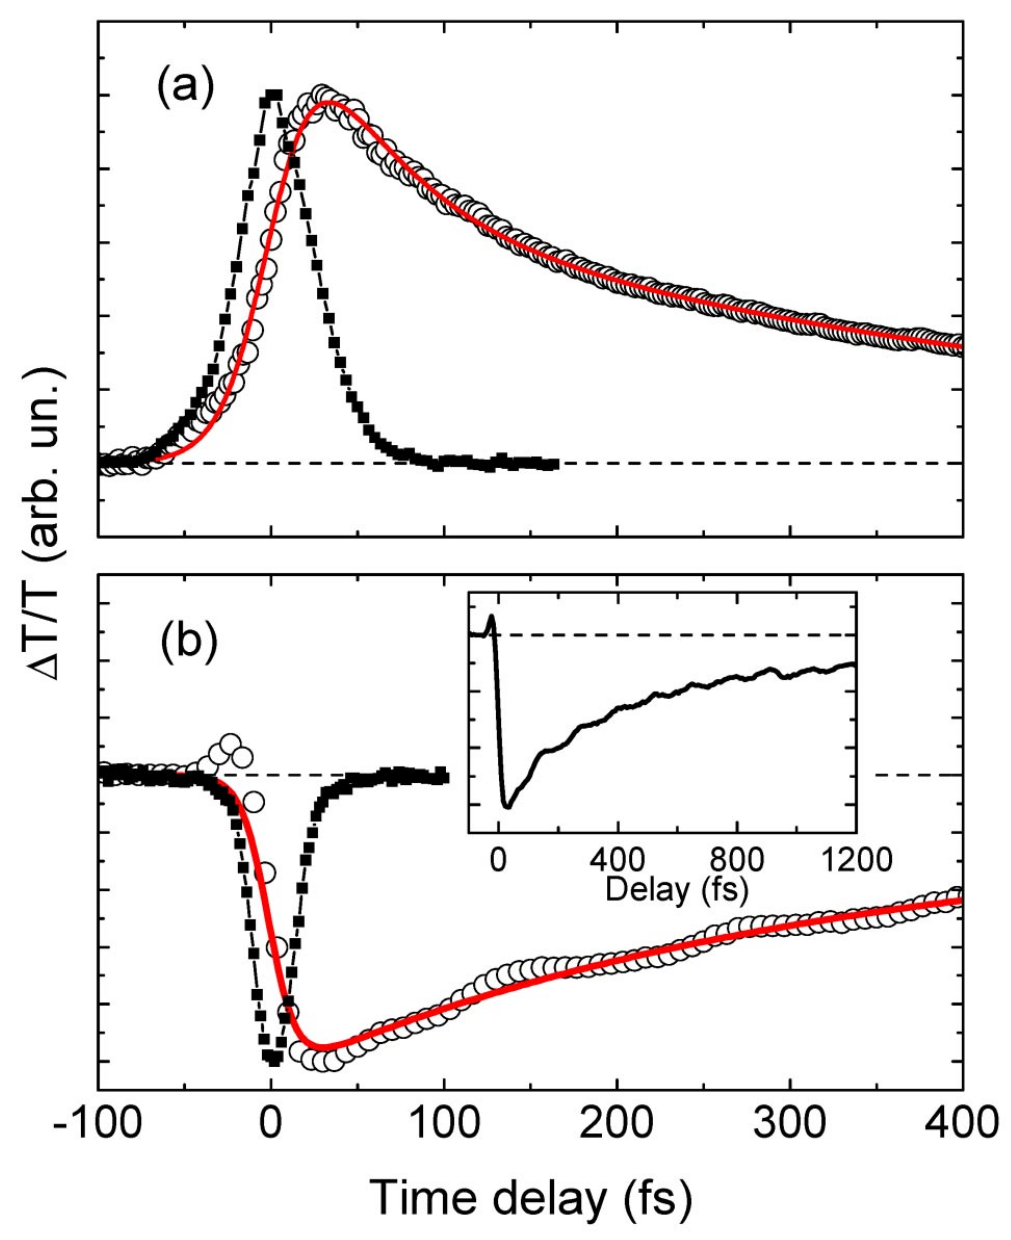
\includegraphics[scale=0.2]{images/chapter_prior_works/e11_pump_probe_manzoni}
	\caption{Carrier relaxation dynamics of SWCNTs photo-excited at 0.92 eV. Under this condition, the two plots correspond to differential transmission probed at 0.92 eV (a) and probed at 2.15 eV (b). The inset figure shows the relaxation measured at 2 eV on a longer time scale. The open circles represent the experimental data, and the solid lines indicate numerical fits to the data. The autocorrelation measurement of the pump pulse is also overlayed on both figures (squares + line). Reproduced from Ref.\ \cite{manzoni2005intersubband}.}
	\label{fig:e11_pump_manzoni}
\end{figure}

\begin{figure}[H]
	\centering
	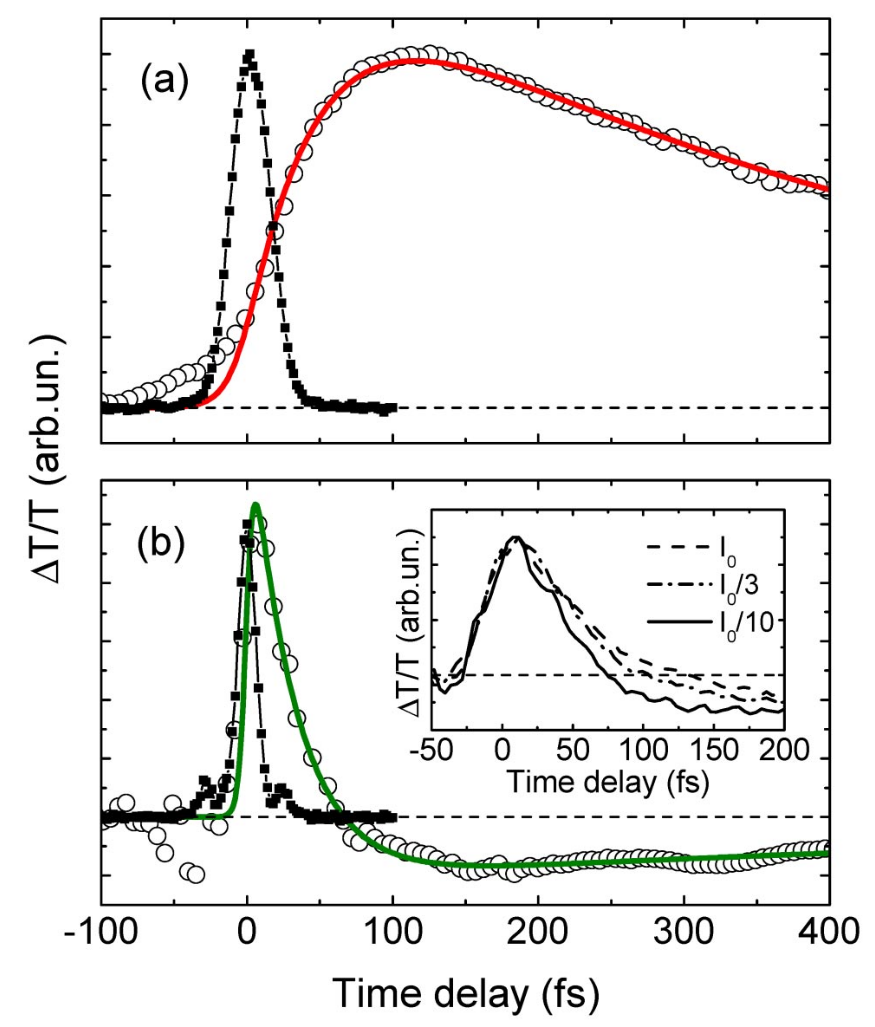
\includegraphics[scale=0.25]{images/chapter_prior_works/e22_pump_probe_manzoni}
	\caption{Carrier relaxation dynamics of SWCNTs photo-excited at 2.15 eV. Under this condition, the two plots correspond to differential transmission probed at 0.95 eV (a) and probed at 2 eV (b). The inset figure shows the pump power dependence measurements of the differential transmission probed at 2 eV. The open circles represent the experimental data, and the solid lines indicate numerical fits to the data. The autocorrelation measurement of the pump pulse is also overlayed on both figures (squares + line). Reproduced from Ref.\ \cite{manzoni2005intersubband}.}
	\label{fig:e22_pump_manzoni}
\end{figure}

\begin{figure}[ht]
	\centering
	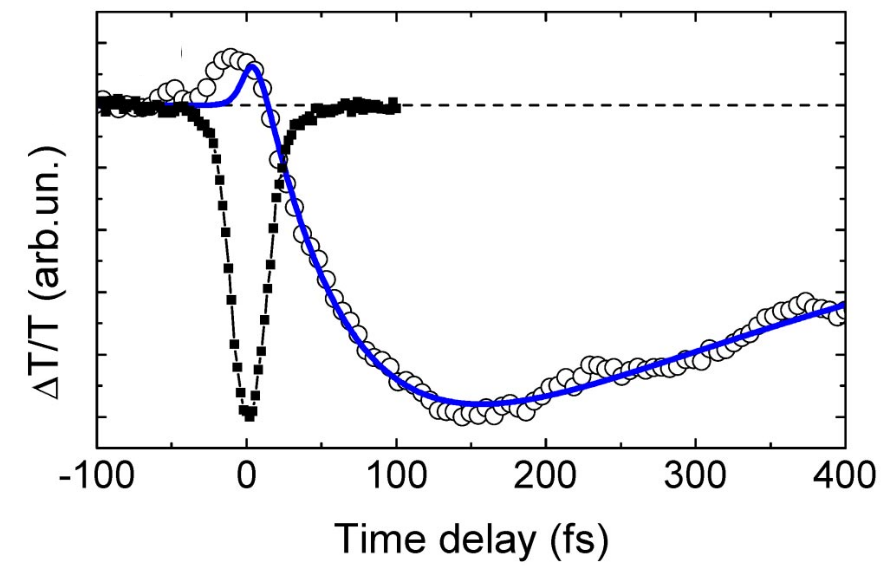
\includegraphics[scale=1.3]{images/chapter_prior_works/e33_pump_e22_probe_manzoni}
	\caption{Carrier relaxation dynamics of SWCNTs photo-excited at 2.75 eV and probed at 2.1 eV. The open circles represent the experimental data, and the solid line indicates a numerical fit to the data. The autocorrelation measurement of the pump pulse is also overlayed on the plot (squares + line). Reproduced from Ref.\ \cite{manzoni2005intersubband}.}
	\label{fig:e33_pump_manzoni}
\end{figure}



\subsection{Ostojic et al.\ (2005)}

In general, excitons are expected to be stable in a scenario where their Bohr radius $r_\text{Bohr}$ is much smaller than the typical inter-exciton distance $d_\text{exc}$ \cite{mott1961transition}. Increasing the density of excitons can establish a condition where $r_\text{Bohr} \approx d_\text{exc}$ once the density is greater than or equal to a critical value known as the Mott density \cite{mott1961transition}. This causes a Mott transition process to occur where screening effects suppress the Coulomb interaction between electrons and holes, causing them to dissociate to create a free electron plasma \cite{mott1961transition}. Ostojic et al.\ (2005) investigated this phenomenon in SWCNTs using non-degenerate, pump-probe spectroscopy \cite{ostojic2005stability} featuring a broadband probe. They claim that even at the Mott density, excitons still remain stable.

\begin{figure}[ht]
	\centering
	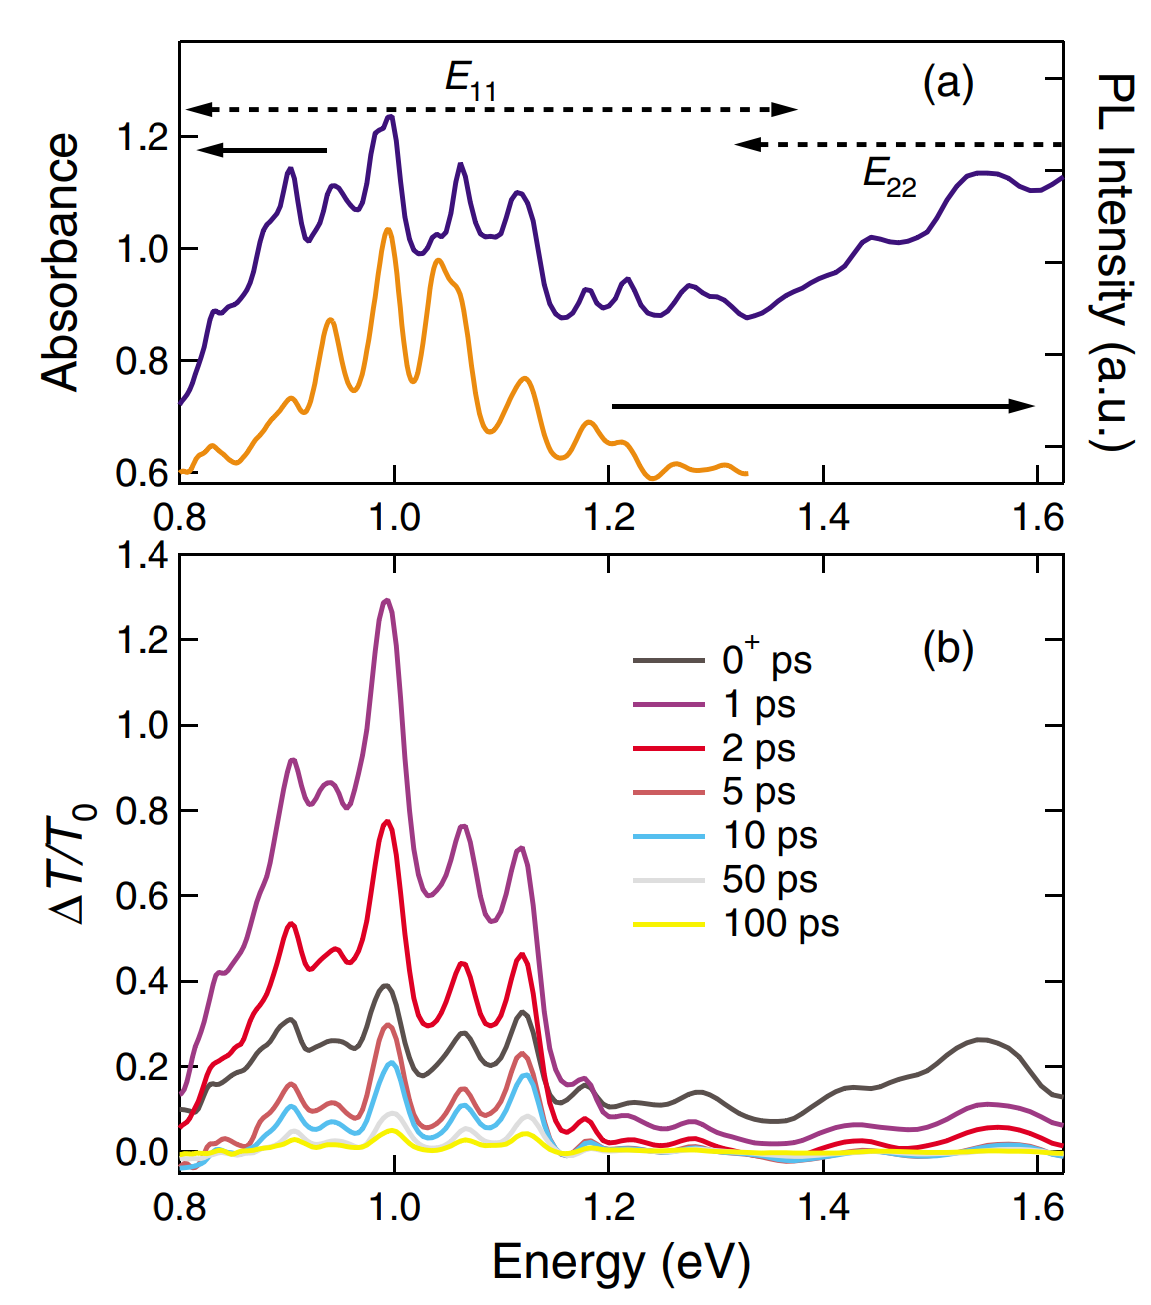
\includegraphics[scale=0.22]{images/chapter_prior_works/abs_dtt_gordana_2005}
	\caption{{\color{red} UNFINISHED} Reproduced from Ref.\ \cite{ostojic2005stability}. }
	\label{fig:abs_dtt_gordana_2005}
\end{figure}

Figure \ref{fig:abs_dtt_gordana_2005} shows the linear absorption and photoluminescence spectra of their HiPCo SWCNT dispersion sample as well as differential transmission data obtained at various time delays. The differential transmission data was taken using an optical pump centered at \SI{775}{\nano\meter}. Within the first \SI{1}{\pico\second}, the signal observed within the $E_{22}$ range appears to decay whereas, that of the $E_{11}$ range increases rapidly. This agrees with the fast inter-subband dynamics observed by Manzoni et al.\ (2005). Moreover, the spectral shape of the differential transmisson stays constant and only changes in amplitude.


\begin{figure}[ht]
	\centering
	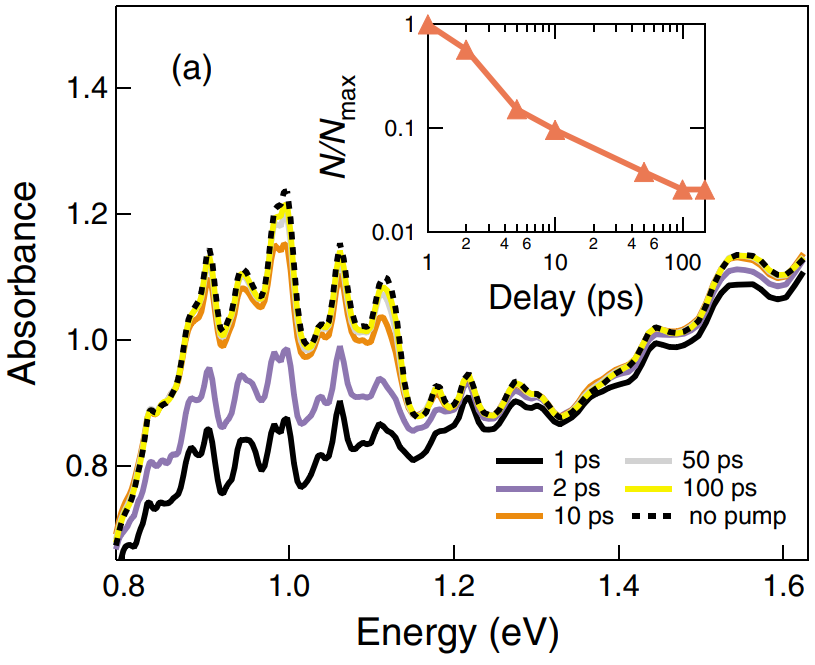
\includegraphics[scale=1.2]{images/chapter_prior_works/total_abs_gordana_2005}
	\caption{{\color{red} UNFINISHED} Reproduced from Ref.\ \cite{ostojic2005stability}.}
	\label{fig:total_abs_gordana_2005}
\end{figure}


These effects can be interpreted more easily by taking the linear absorption of the sample into account. Hence, Figure \ref{fig:total_abs_gordana_2005} shows how the total absorbance of the sample changes. The absorption associated with excitonic resonances decreases due to photo-bleaching effects. However, the overall shape of these resonances appears t remain constant. The peak positions do not shift in energy either.

Ostojic et al.\ (2005) estimate the number of photo-excited excitons in nanotubes by taking into account the total number of nanotubes within the photo-excited volume of their sample, the change in absorbance, as well as the pump fluence. They deduce that the density of excitons in a typical nanotube of length \SI{150}{\nm} is on the order of $5 \times 10^6$ \si{\per\cm}. This yields an average seperation of \SI{2}{\nm} between excitons. In addition, they acknowledge that theoretical calculations in the literature that suggest that the typical Bohr radius in SWCNTs of diameter 1 nm range between 2 - 5 \si{\nm}.

Estimates such as these imply that that shortly after photoexcitation, the optical pump creates enough excitons such that a Mott transition may indeed occur as the Bohr radius is of the same order of magnitude as the average inter-exciton distance. However, the presence that exciton resonances even at high pump fluences shows that excitons have not yet dissociated to form a free-electron plasma. Experimental results such as these have raised questions as to whether it is even possible to reach the Mott density in SWCNTs. Indeed, a number of studies have presented evidence that efficient exciton-exciton annihilation processes in SWCNTs establish an upper limit on the density of excitons that is below the Mott density.


\section{Reports of Exciton-Exciton Annihilation}

{\color{red} ADD INTRO PARAGRAPH FOR THIS SECTION}

\begin{equation}
\label{eq:exc_annih}
\ce{X + X $\rightarrow$ X},
\end{equation}

\subsection{Wang et al.\ (2004)}
{\color{red} UNFINISHED}
Wang et al.\ (2004) observed non-linear recombination dynamics in time-resolve fluorescence experiments \cite{wang2004observation}. Measured a dispersion of HiPco SWCNTs. Figure \ref{fig:fluorescence_wang_2004} shows results. At higher pump fluences, the onset of a fast exponential decay process becomes more prominent. This behavior exemplifies a well-known signature of Auger recombination processes. In addition, the fluorescence observed at longer time delays appears to saturate as shown in the inset plot of Figure \ref{fig:fluorescence_wang_2004}.



Furthermore, Figure \ref{fig:fast_slow_wang_2004} shows the time-integrated fluoresence contributions associated with the fast and slow decays. The fluorescence from the slow decay begins saturating at fluences greater than \SI{0.3}{\joule / \meter\squared}. In contrast, the time-integrated fluoresence linked with the fast decay only begins to saturate at a fluence of \SI{1.5}{\joule / \meter\squared}. These data suggest that exciton-exciton annihilation associated with the fast decay process establishes an upper limit of bright excitons that can exist at longer time delays.




Wang et al.\ interpreted these results by devising a model of carrier dynamics that accounts for Auger recombination processes. They postulate that the time-dependent, probability distribution of a nanotube having $N$ electron-pairs $\rho^\text{N}(t)$ depends on the rate of radiate emission $\gamma^\text{N}_\text{r}$, the rate of Auger recombination $\gamma^\text{N}_\text{A}$, as well as the rate of carrier trapping at defects $\gamma_\text{t}$. The master equation
\begin{equation}
	\dfrac{\mathrm{d}\rho^\text{N}}{\mathrm{d} t} = \rho^\text{N}(\gamma^\text{N+1}_\text{r} + \gamma^\text{N+1}_\text{A} + \gamma_\text{t})(N+1) - \rho^\text{N}(\gamma^\text{N}_\text{r} + \gamma^\text{N}_\text{A} + \gamma_\text{t})N,
\end{equation}
captures the relationship between these quantities. In the case of excitons,
\begin{equation}
	\gamma^\text{N}_\text{r} = \text{const}, \text{   } \gamma^\text{N}_\text{A} = C_\text{A}(N-1),
\end{equation}
where $C_\text{A}$ is the Auger rate coefficient. Initial population of excitons $N_\text{initial} = \phi \sigma$, where $\phi$ and $\sigma$ denote, respectively, the fluence of the optical pump and the absorption cross-section of carbon nanotubes. Indeed the qualitative results from this model agree with the experimental data presented in Figures \ref{fig:fluorescence_wang_2004} and \ref{fig:fast_slow_wang_2004}.

Numerical fits to the data yield an estimate of $C_\text{A}$ which was found to be $\SI{0.8}{\per\pico\second}$. Correspondingly, this also provides an estimate of the typical lifetime of excitons that participate in exciton-exciton annihilation given as $1/\gamma^\text{N}_\text{A}$ which was determined to be on the order of picoseconds with lifetimes being as short as \SI{1.2}{\pico \second}.

\begin{figure}[ht]
	\centering
	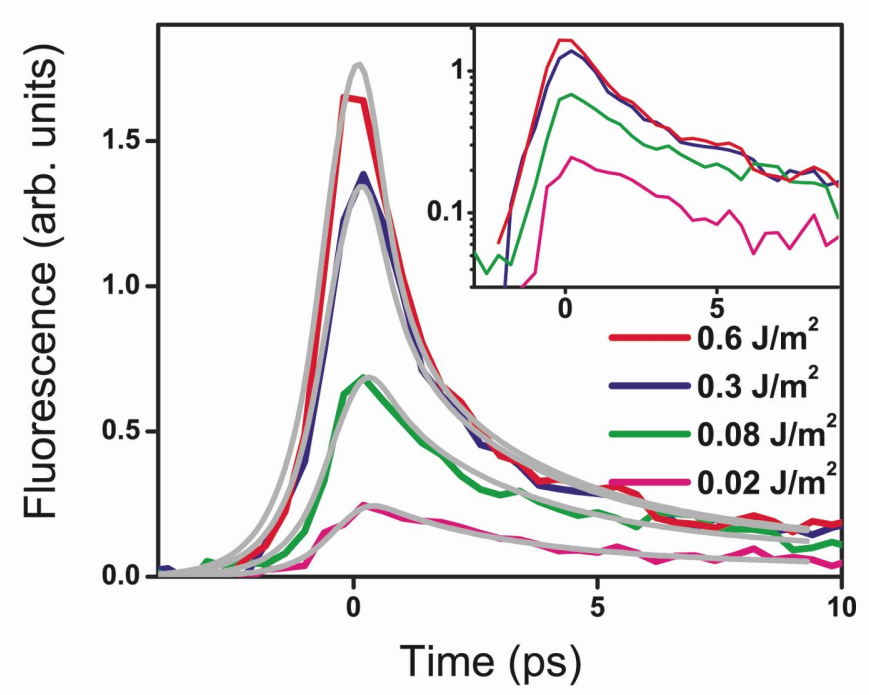
\includegraphics[scale=0.25]{images/chapter_prior_works/fluorescence_wang_2004}
	\caption{Time-resolved fluorescence captured at indicated fluences. The gray curves are fits to the experimental data using a model based on exciton-exciton annihilation. At higher fluences, the dynamics exhibit a bi-exponential decay containing a fast and a slow process. The fast exponential decay has been attributed to the presence of a non-radiative decay mechanism associated with exciton-exciton annihilation whereas, the slow component emerges due to radiative inter-band recombination. The inset figure shows the same experimental data on a log-linear plot to emphasize the saturation of the fluoresence at higher pump fluences occuring due to non-radiative decay phenomena. Reproduced from Ref.\ \cite{wang2004observation}.}
	\label{fig:fluorescence_wang_2004}
\end{figure}

\begin{figure}[ht]
	\centering
	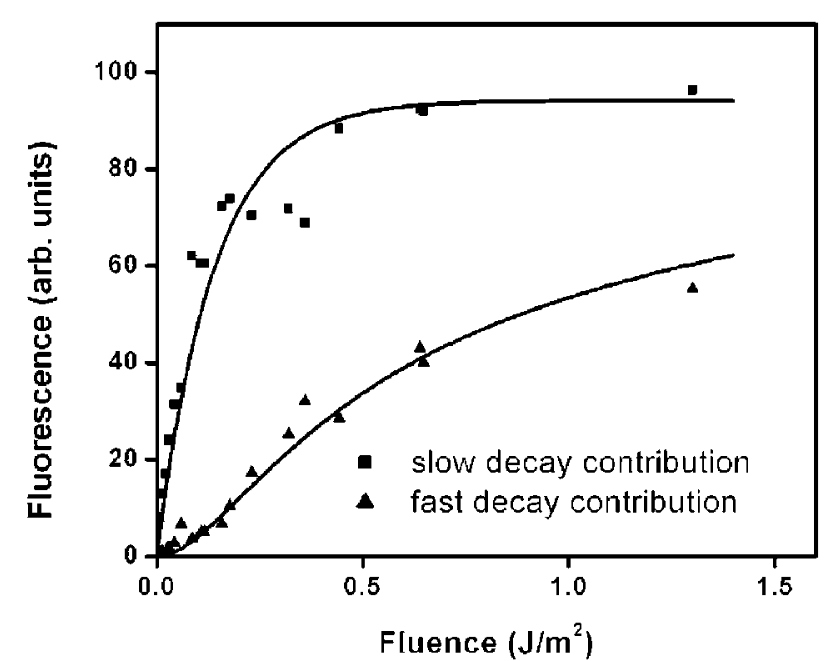
\includegraphics[scale=0.3]{images/chapter_prior_works/fast_slow_wang_2004}
	\caption{Time-integrated fluorscence associated with fast and slow decay contributions as a function of pump fluence. The solid curves represent fits to the data. The fluorescence associated with the slow decay saturates at a fluence above \SI{0.3}{\joule / \meter \squared}, indicating an upper limit of bright excitons. However, the time-integrated fluorescence of the fast decay only begins to saturate at 1.5  \SI{1.5}{\joule / \meter \squared}. Reproduced from Ref.\ \cite{wang2004observation}.}
	\label{fig:fast_slow_wang_2004}
\end{figure}





\subsection{Ma et al.\ (2004)}

{\color{red} UNFINISHED}
Ma et al.\ (2004) also obtained experimental results that qualtitatively agree with those observed by Wang et al. Also measured dispersion of HiPCo SWCNTs.

Used the rate equation
\begin{equation}
	\dfrac{\mathrm{d}N(t)}{\mathrm{d}t} = - k N(t) - \gamma N(t)^2,
\end{equation}
to characterize carrier dynamics. If $kt < 1$, this gives analytical solution
\begin{equation}
	N(t) = \dfrac{N(0)}{1 + N(0)\gamma \cdot t}
\end{equation}

Assume that time-dependent, fluorescence intensity $I(t) \propto N(t)$ to obtain
\begin{equation}
  	\left( \dfrac{I(t)}{I_0} \right)^{-1} \approx \left( \dfrac{N(t)}{N_0} \right)^{-1} = \gamma N(0) \cdot t + 1
\end{equation}

\begin{figure}[ht]
	\centering
	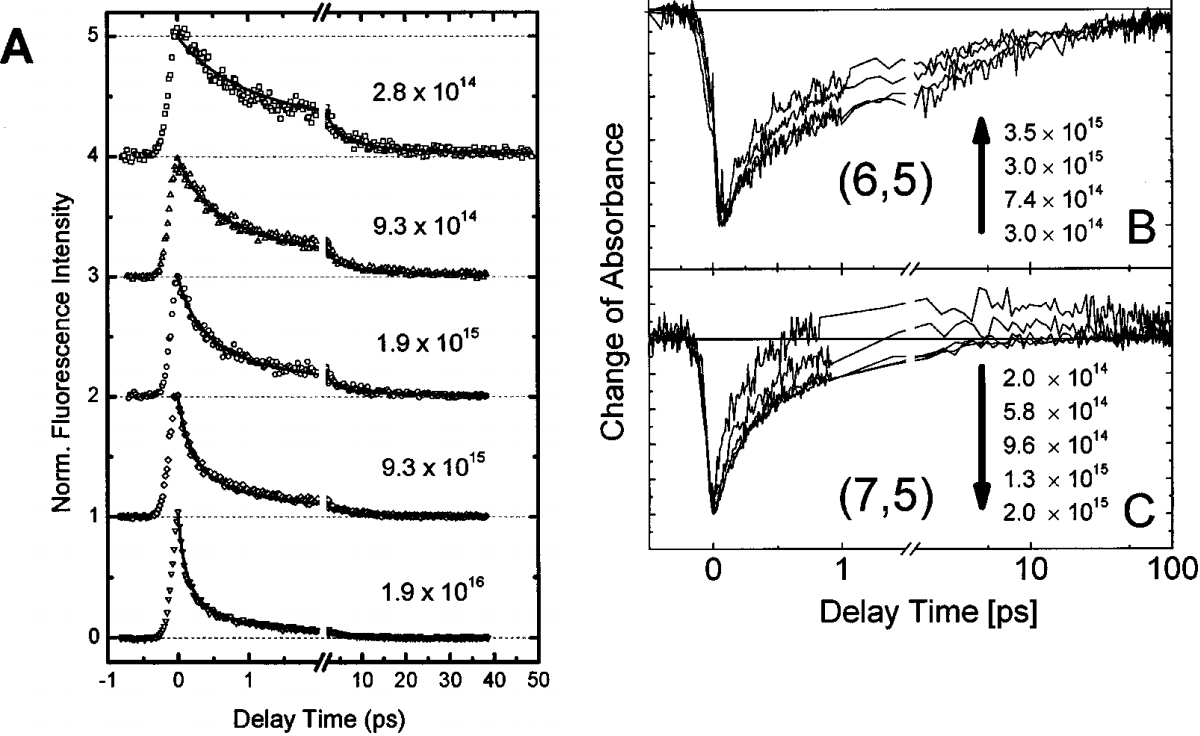
\includegraphics[scale=1.4]{images/chapter_prior_works/fluorescence_abs_ma_2004}
	\caption{{\color{red} UNFINISHED} Reproduced and modified from Ref.\ \cite{ma2004ultrafast}.}
\end{figure}

\subsection{Ma et al.\ (2005)}

Reference \cite{ma2005femtosecond}.

\begin{figure}[ht]
	\centering
	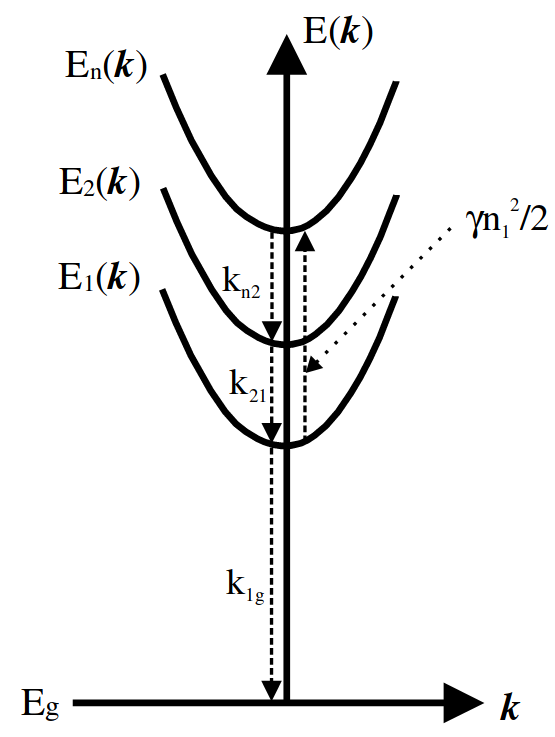
\includegraphics[scale=0.3]{images/chapter_prior_works/exciton_schematic_ma_2005}
	\caption{{\color{red} UNFINISHED} Reproduced from Ref.\ \cite{ma2005femtosecond}.}
\end{figure}

\begin{figure}[ht]
	\centering
	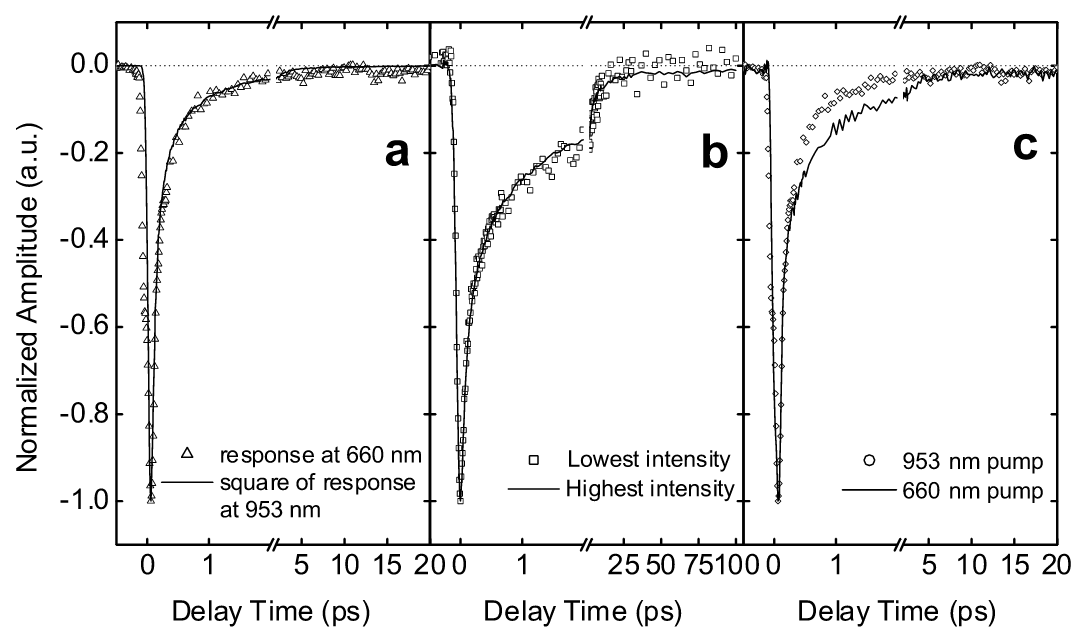
\includegraphics[scale=0.4]{images/chapter_prior_works/abs_ma_2005}
	\caption{{\color{red} UNFINISHED} Reproduced from Ref.\ \cite{ma2005femtosecond}.}
\end{figure}

\subsection{Valkunas et al.\ (2006)}
{\color{red} UNFINISHED} Valkunas et al.\ (2006) use exciton manifold to derive a set of rate equations used to model carrier dynamics, including exciton-exciton annihilation \cite{valkunas2006exciton}.

\begin{figure}[ht]
	\centering
	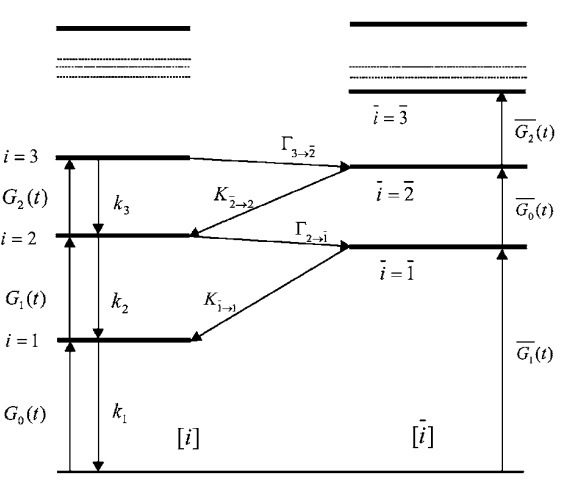
\includegraphics[scale=0.5]{images/chapter_prior_works/exciton_manifold_valkunas_2006}
	\caption{ {\color{red} UNFINISHED} Reproduced from Ref.\ \cite{valkunas2006exciton}. }
	\label{fig:exciton_manif_valkunas}
\end{figure}

\subsection{Luer et al (2009)}
Reference \cite{luer2009size}

\subsection{Murakami et al.\ (2009)}
{\color{red} UNFINISHED} Efficient exciton-exciton annihilation \cite{murakami2009existence}.



%\section{Possible Presence of Bi-excitons and Trions}

%non-degenerate pump-probe. Amplified Ti:sapphire laser operating at 200 KHz and pulse duration of 100 fs. Probe generated using supercontinuum generation in a sapphire crystal. Pump generated using optical parametric amplifier (OPA). Studied a (6,5)-enriched dispersion. Figure \ref{fig:abs_yuma} shows linear absorption spectrum of sample.

%\begin{figure}[ht]
%	\centering
%	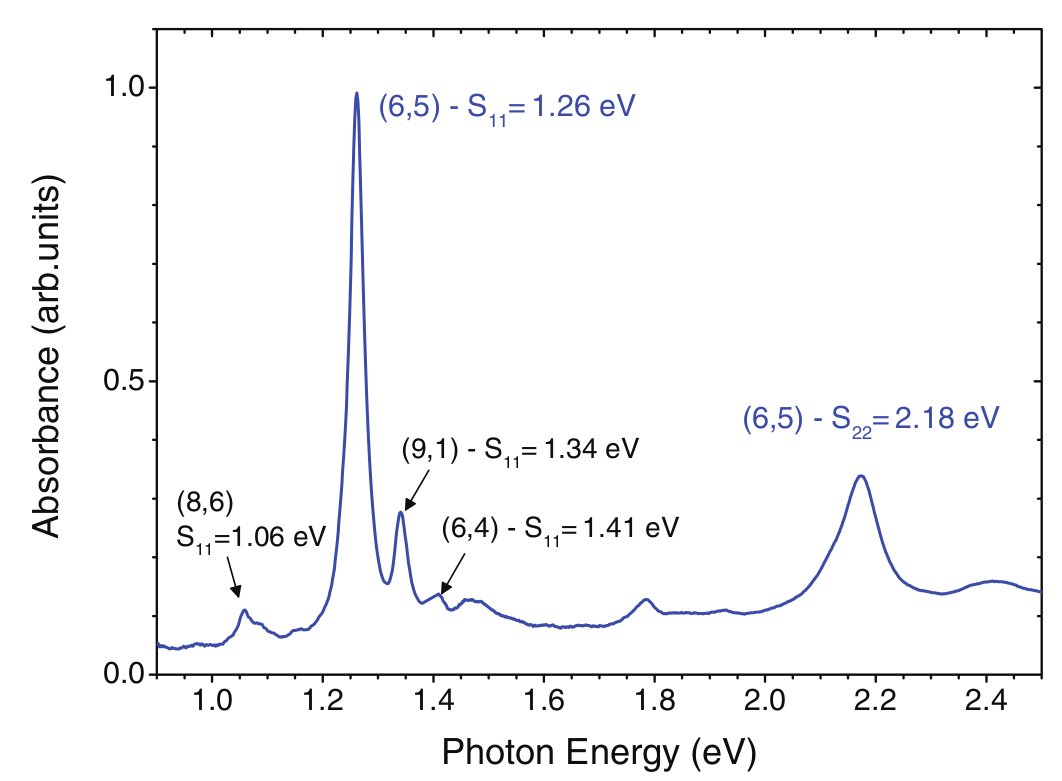
\includegraphics[scale=0.3]{images/chapter_prior_works/abs_yuma}
%	\caption{Slightly different nomenclature. Here, $S_\text{ij} \equiv E_\text{ij}$.  Reproduced from Ref.\ \cite{yuma2013biexciton}.}
%	\label{fig:abs_yuma}
%\end{figure}

%Figure \ref{fig:dtt_yuma} shows experimental data after resonantly exciting $E_{22}$ transition of (6,5) nanotube. Notice photo-bleaching and a blue shift occuring at $E_{11}$ peak. Interpreted as excitons occupying $E_{11}$ states. Charge screening due to Coulomb interactions between excitons blueshifts exciton peak. State that initial sharp decay due to exciton-exciton annihilation.

%Observed photo-induced absorption at 1.13 eV. Attribute this to the formation of biexcitons. Provided additional evidence by pumping at and below $E_{11}$. When pumping below $E_{11}$, photo-induced absorption at 1.13 eV recedes. When pumping $E_{11}$ resonantly, photo-induced absorption becomes more significant indicating that it may be directly associated with (6,5). Carrier dynamics at $E_{11}$ and bi-exciton appear to be correlated with each other.

%\begin{figure}[ht]
%	\centering
%	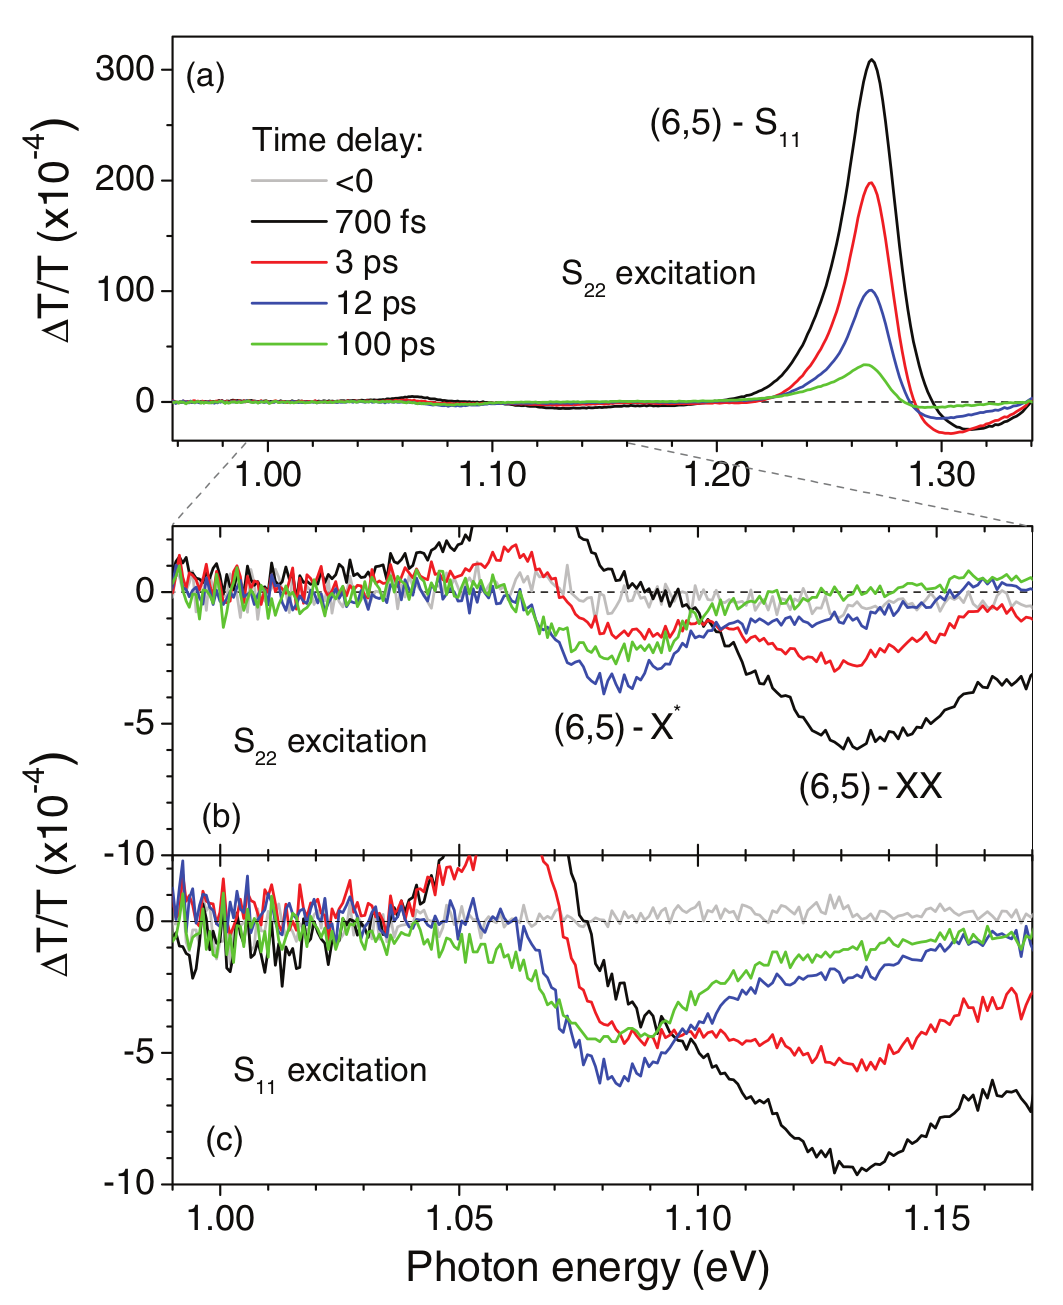
\includegraphics[scale=0.3]{images/chapter_prior_works/dtt_yuma}
%	\caption{{\color{red} UNFINISHED} Reproduced from Ref.\ \cite{yuma2013biexciton}.}
%	\label{fig:dtt_yuma}
%\end{figure}


%Exciton-Exciton annihilation \cite{valkunas2006exciton, yuma2013biexciton}.
%They also show that exciton-exciton annihilation occurs over a time scale such that it is hard to reach Mott densitty of excitons where excitons immediately dissociate to form plasma of free carriers. These a
%Apparently, excitons dissociate into free electron-hole pairs before recombination occurs \cite{kumamoto2014spontaneous}.


\section{Optical Stark Effect}
{\color{red} UNFINISHED}

\subsection{Song et al.\ (2006)}
Ref.\ \cite{song2006optical}.

\subsection{Maeda et al.\ (2006)}

\begin{figure}[ht]
	\centering
	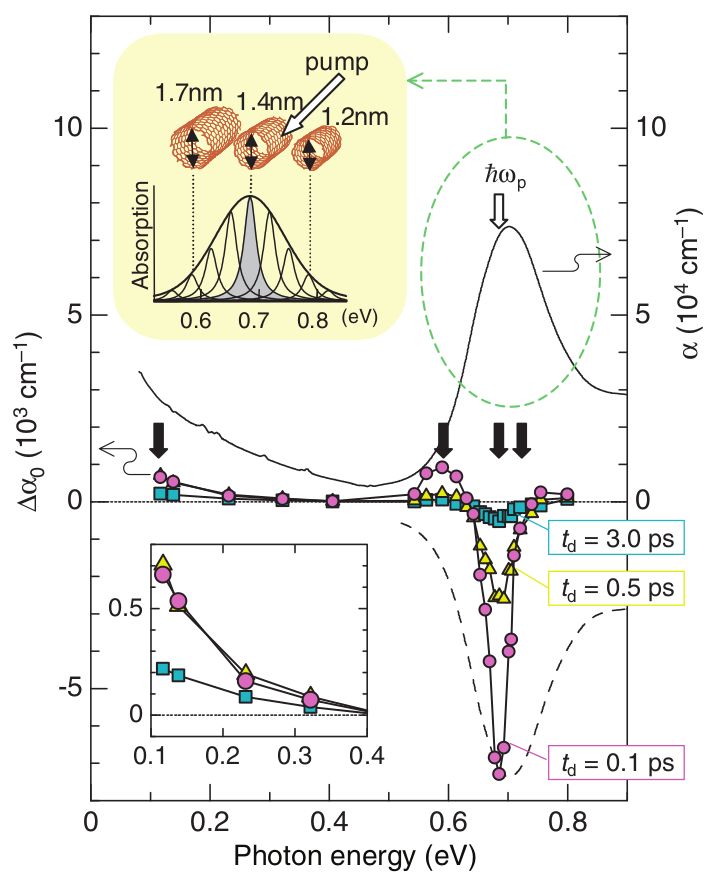
\includegraphics[scale=0.4]{images/chapter_prior_works/stark_shift_maeda}
	\caption{{\color{red} UNFINISHED} Reproduced from Ref.\ \cite{maeda2006gigantic}.}
\end{figure}

\subsection{Matsumoto et al.\ (2006)}

Ref.\ \cite{matsumoto2006optical}.

\subsection{Tao et al.\ (2009)}

Ref. \cite{tao2009subpicosecond}.

\section{Summary}
